%!TEX TS-program = xelatex
\documentclass[12pt, a4paper]{article}  

\usepackage{etex} % расширение классического tex в частности позволяет подгружать гораздо больше пакетов, чем мы и займёмся далее

%%%%%%%%%% Математика %%%%%%%%%%
\usepackage{amsmath,amsfonts,amssymb,amsthm,mathtools} 
%\mathtoolsset{showonlyrefs=true}  % Показывать номера только у тех формул, на которые есть \eqref{} в тексте.
%\usepackage{leqno} % Нумерация формул слева


%%%%%%%%%%%%%%%%%%%%%%%% Шрифты %%%%%%%%%%%%%%%%%%%%%%%%%%%%%%%%%
\usepackage{fontspec}         % пакет для подгрузки шрифтов
\setmainfont{Arial}   % задаёт основной шрифт документа

\defaultfontfeatures{Mapping=tex-text}

% why do we need \newfontfamily:
% http://tex.stackexchange.com/questions/91507/
\newfontfamily{\cyrillicfonttt}{Arial}
\newfontfamily{\cyrillicfont}{Arial}
\newfontfamily{\cyrillicfontsf}{Arial}
\usepackage{unicode-math}     % пакет для установки математического шрифта
\setmathfont{Asana Math}      % шрифт для математики
% \setmathfont[math-style=ISO]{Asana Math}
% Можно делать смену начертания с помощью разных стилей
\renewcommand{\thefigure}{\thesection:\arabic{figure}}
\renewcommand{\theequation}{Eq.~(\arabic{equation})}
% Конкретный символ из конкретного шрифта
% \setmathfont[range=\int]{Neo Euler}

\usepackage{polyglossia}      % Пакет, который позволяет подгружать русские буквы
\setdefaultlanguage{russian}  % Основной язык документа
\setotherlanguage{english}    % Второстепенный язык документа


%%%%%%%%%% Работа с картинками %%%%%%%%%
\usepackage{graphicx}                  % Для вставки рисунков
\usepackage{graphics}
\graphicspath{{pop-art/}} 
\graphicspath{{DataFest_Stikers/}}    % можно указать папки с картинками
\usepackage{wrapfig}                   % Обтекание рисунков и таблиц текстом
\usepackage{subfigure}                 % для создания нескольких рисунков внутри одного
\DeclareGraphicsExtensions{.pdf,.png,.jpeg,.jpg}

%%%%%%%%%% Работа с таблицами %%%%%%%%%%
\usepackage{tabularx}            % новые типы колонок
\usepackage{tabulary}            % и ещё новые типы колонок
\usepackage{array}               % Дополнительная работа с таблицами
\usepackage{longtable}           % Длинные таблицы
\usepackage{multirow}            % Слияние строк в таблице
\usepackage{float}               % возможность позиционировать объекты в нужном месте
\usepackage{booktabs}            % таблицы как в книгах!
\renewcommand{\arraystretch}{1.3} % больше расстояние между строками

% Заповеди из документации к booktabs:
% 1. Будь проще! Глазам должно быть комфортно
% 2. Не используйте вертикальные линни
% 3. Не используйте двойные линии. Как правило, достаточно трёх горизонтальных линий
% 4. Единицы измерения - в шапку таблицы
% 5. Не сокращайте .1 вместо 0.1
% 6. Повторяющееся значение повторяйте, а не говорите "то же"
% 7. Есть сомнения? Выравнивай по левому краю!

%%%%%%%%%% Графика и рисование %%%%%%%%%%
\usepackage{tikz, pgfplots}  % язык для рисования графики из latex'a
\usepackage{amscd}                  %Пакеты для рисования
\usepackage[matrix,arrow,curve]{xy} %комунитативных диаграмм
\usepackage{xcolor}
\usepackage[ampersand]{easylist}
\usepackage{ccaption}
\captiondelim{ } % убирает двоеточие в конце
\DeclareMathOperator{\Var}{Var}
\DeclareMathOperator{\Cov}{Cov}


\title{Домашняя работа № 3.1.\\ Свои собственные}
\date{\today}

\begin{document}
\maketitle

\section{Создайте такие математический операторы, как Var и Cov}
\Large{\textbf{\textcolor{blue}{Математический оператор для дисперсии}}} \\
\Large{$\Var$}\\
\textbf{\textcolor{blue}{Математический оператор для ковариации}} \\
\Large{$\Cov$}

\section{Вы всё время по ходу текста должны писать $\sigma$-
алгебра. Напишите команду, которая позволит делать это без
перехода в математический режим. Например, s-алгебра.}
\Large{\textbf{\textcolor{blue}{Сигма - алгебра:}}}\\
\def\s{\ensuremath{\sigma}}
\s-алгебра

\section{Написать команду, которая будет выводить $x_1 \ldots x_n$}
\Large{\textbf{\textcolor{blue}{Последовательность:}}} \\
\newcommand{\vect}{\ensuremath{x_1 \ldots x_n}}
\vect

\section{Усовершенствовать предыдущую команду. Она должна быть
от двух аргументов и при запросе com{a}{z}, com{1}{6} и
com{(a,b)}{(c,d)} выдавать соответственно 
$x_a \ldots x_z, 
x_1 \ldots x_6, 
x_{(a,b)} \ldots x_{(c,d)}$}
\newcommand{\com}[2]{\ensuremath{x_#1 \ldots x_#2}}
\com{a}{z}\\
\com{1}{6}\\
\com{{(a,b)}}{{(c,d)}}

\section{ Сделать так, чтобы в itemize каждый новый пункт шёл после синей точки}


\begin{itemize}
\item [\textcolor{blue}{$\bullet$}]\textit{Первый пункт}
\item [\textcolor{blue}{$\bullet$}]\textit{Второй пункт}
\item [\textcolor{blue}{$\bullet$}]\textit{Третий пункт}
\end{itemize}

\section{Заменяем пределы}
Было:
\[\lim_{x \to 0} \frac{\sin{x}}{x}  \]
Стало:\\
\def\llim{\begin{center}
\ensuremath{\displaystyle\lim\limits_{x \to 0} \frac{\sin{x}}{x}}
\end{center}}
\llim
Переопределение предела:\\
\renewcommand{\L}{\lim}
\begin{center}{$\displaystyle\L\limits_{x \to 0} \frac{\sin{x}}{x}$}\
\end{center}

\section{Сделайте нумерацию рисунков в документе в следующемформате: "номер секции: номер рисунка". Обязательноприложите к файлу рисунок, который вы будете использовать для демонстрации своих достижений.}
\begin{figure} [H]
\begin{center}
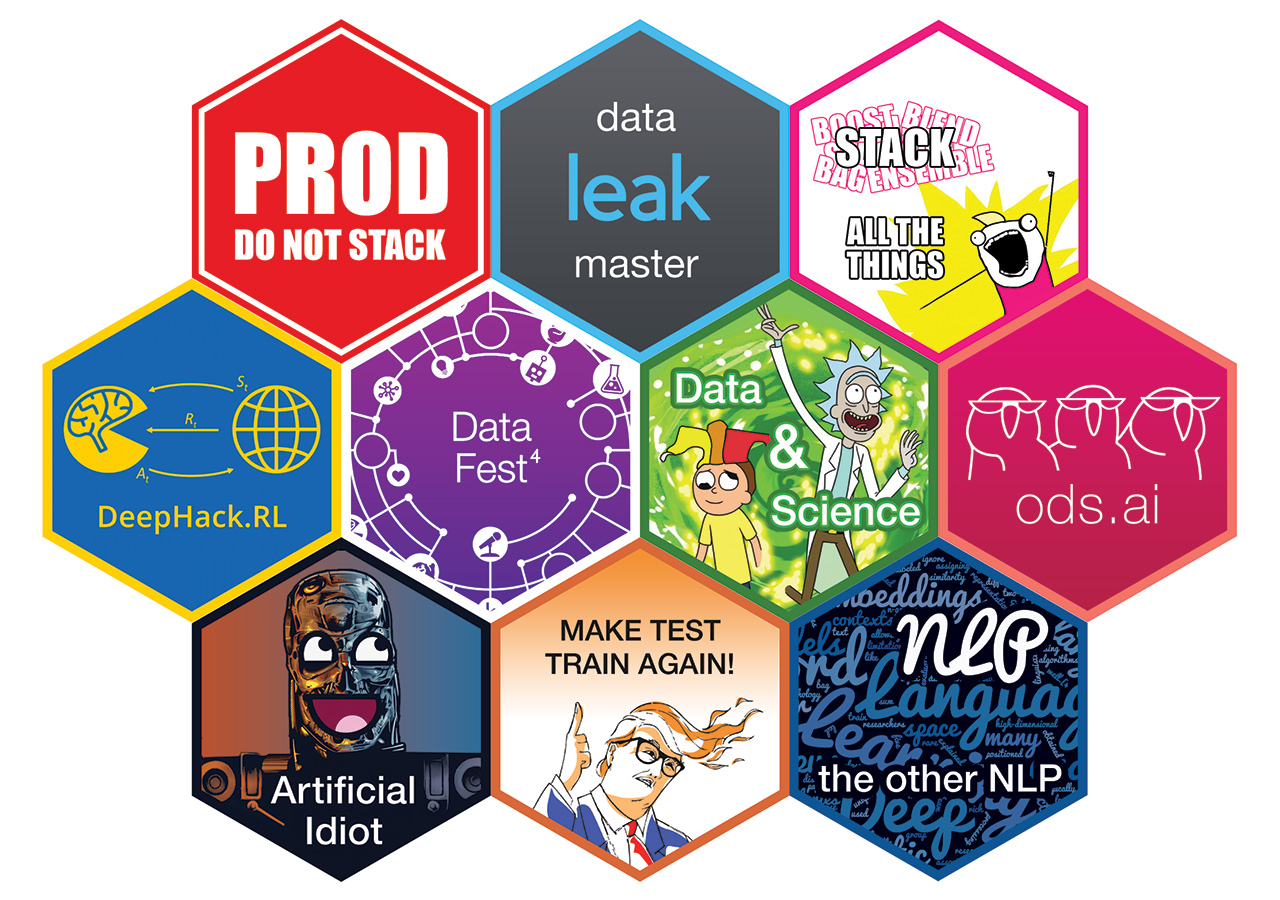
\includegraphics[scale=0.15]{1.jpg} 
\end{center}
\caption{}
\end{figure}

\begin{figure} [H]
\begin{center}

\includegraphics[scale=0.15]{f.jpg} 
\end{center}
\caption{}
\end{figure}

\section{перенумеруем формулы}

\begin{equation}
D= \frac{\rho_b}{\rho_{bs}} \times 100 
\end{equation}

\begin{equation}
S_n = \sum_{i=1}^{n} \frac{b_1(1-q^n)}{1 - q}
\end{equation}

\section{Игра с текстом. перевёрнутые буквы}

\newcommand{\ex}[2]{
\ifnumcomp{#1}{=}{1}{\rotatebox{180}{\textcolor{green}{#2}}}{\ifnumcomp{#1}{=}{2}{\reflectbox{\textcolor{pink}{#2}}}{ \reflectbox{\rotatebox{180}{\textcolor{purple}{#2}}}}}}

\newcommand{\exu}[2]{
\ifstrequal{#1}{поворот}{\rotatebox{180}{\textcolor{green}{#2}}}{\ifstrequal{#1}{зеркало}{\reflectbox{\textcolor{pink}{#2}}}{ \reflectbox{\rotatebox{180}{\textcolor{purple}{#2}}}}}}

%Есть три режима
%1 - поверни текст
%2 - зеркально отобрази
%3 - сделай всё сразу
%Либо пиши латеху, то что ты хочешь сделать с текстом
%поворот - поверни текст
%зеркало - зеркально отобрази
%вместе - сделай всё сразу

%\ex{2}{привет}
\exu{вместе}{пока}

\end{document}

